% Slide template for the FreeBSD Developer Summit.
% Take it or leave it :-)
%
% It requires LaTeX and LaTeX Beamer [1] to compile.
% pdfLaTeX is recommended for compilation as it produces
% PDF file immediately.
%
% $ pdflatex some.latex
%
%
% It is also recommended to convert images to PDF
% by using ImageMagick ("convert") before including them.
%
% [1] http://latex-beamer.sourceforge.net
%

\documentclass{beamer}

\usepackage{url}
\usepackage[english]{babel}
\usepackage{verbatim}
\usepackage{graphicx}
\usepackage{listings}
\usepackage{mathtools}
\usepackage{color}
\usepackage{listings}

\mode<presentation>
{
  \definecolor{beamer@gker}{rgb}{0.8,0.0,0.0}
  \setbeamercolor*{structure}{fg=beamer@gker}
  \logo{
\includegraphics[scale=0.5]{logo.pdf}}
}

\setbeamertemplate{footline}[text line]{%
  \parbox{\linewidth}{\vspace*{-8pt}
  \prestitle
  \hfill
  \insertshorttitle
  \hfill
  \insertframenumber\ of \inserttotalframenumber}}
\setbeamertemplate{navigation symbols}{}

\definecolor{light-gray}{gray}{0.60}

\lstdefinestyle{custommake}{
  belowcaptionskip=1\baselineskip,
  breaklines=true,
  frame=L,
  xleftmargin=\parindent,
  language=Make,
  showstringspaces=false,
  basicstyle=\footnotesize\ttfamily,
  keywordstyle=\bfseries\color{green!40!black},
  commentstyle=\itshape\color{purple!40!black},
  identifierstyle=\color{blue},
  stringstyle=\color{orange},
}

\definecolor{mygreen}{rgb}{0,0.6,0}
\definecolor{mygray}{rgb}{0.5,0.5,0.5}
\definecolor{mymauve}{rgb}{0.58,0,0.82}



\lstset{ %
  backgroundcolor=\color{white},   % choose the background color; you must add \usepackage{color} or \usepackage{xcolor}
  basicstyle=\ttfamily\tiny,        % the size of the fonts that are used for the code
  breakatwhitespace=false,         % sets if automatic breaks should only happen at whitespace
  breaklines=true,                 % sets automatic line breaking
  captionpos=b,                    % sets the caption-position to bottom
  commentstyle=\color{mygreen},    % comment style
  deletekeywords={...},            % if you want to delete keywords from the given language
  escapeinside={\%*}{*)},          % if you want to add LaTeX within your code
  extendedchars=true,              % lets you use non-ASCII characters; for 8-bits encodings only, does not work with UTF-8
  frame=single,                    % adds a frame around the code
  keepspaces=true,                 % keeps spaces in text, useful for keeping indentation of code (possibly needs columns=flexible)
  keywordstyle=\color{blue},       % keyword style
  language=Make,                 % the language of the code
  morekeywords={*,...,.include},            % if you want to add more keywords to the set
  numbers=left,                    % where to put the line-numbers; possible values are (none, left, right)
  numbersep=5pt,                   % how far the line-numbers are from the code
  numberstyle=\tiny\color{mygray}, % the style that is used for the line-numbers
  rulecolor=\color{black},         % if not set, the frame-color may be changed on line-breaks within not-black text (e.g. comments (green here))
  showspaces=false,                % show spaces everywhere adding particular underscores; it overrides 'showstringspaces'
  showstringspaces=false,          % underline spaces within strings only
  showtabs=false,                  % show tabs within strings adding particular underscores
  stepnumber=1,                    % the step between two line-numbers. If it's 1, each line will be numbered
  stringstyle=\color{mymauve},     % string literal style
  tabsize=8,                       % sets default tabsize to 2 spaces
  title=\lstname                   % show the filename of files included with \lstinputlisting; also try caption instead of title
}

%%\lstset{escapechar=@,style=custommake}


\usepackage{CJKutf8}
\newcommand{\prestitle}{AsiaBSDCon 2015}

\title{FreeBSD: 5 years of pkg}
\subtitle{A end less journey}
\author{Baptiste Daroussin \\ \url{bapt@FreeBSD.org}}
\institute{
\includegraphics[scale=0.5]{../template/logo.pdf}}
\date{AsiaBSDCon 2015 \\ Tokyo \\ December 13st, 2014}

\begin{document}
\begin{frame}[plain]
	\titlepage
\end{frame}

{
\usebackgroundtemplate{
\begin{picture}(0,0)
\put(180,-180){

\includegraphics[width=2.5in]{starre10.png}
}
\end{picture}
}%
\begin{frame}
	\frametitle{Once upon a time... the binary packages\\\begin{CJK}{UTF8}{min}昔々...バイナリパッケージ\end{CJK}}
	From the package point of view
	\begin{itemize}
		\item No binary upgrade
		\item Inconsistencies
		\item Lots of failing scripts
		\item No signing support
		\item No predictable updates
		\item Sacrifice of chicken mandatory
		\item DO NOT EVER TOUCH AGAIN WHEN YOU MANAGE TO INSTALL
	\end{itemize}
\end{frame}
}

\begin{frame}
	\frametitle{Once upon a time... the binary packages\\\begin{CJK}{UTF8}{min}昔々...バイナリパッケージ\end{CJK}}
	Other OS:
	\begin{itemize}
		\item NetBSD:
			\begin{itemize}
				\item pkg\_tools == pkg\_install++
				\item no library
				\item pkgin tight to pkg\_tools
			\end{itemize}
		\item OpenBSD:
			\begin{itemize}
				\item pkg\_add: full featured
				\item closely tight to OpenBSD's ports tree
				\item perl (not in base on FreeBSD)
			\end{itemize}
		\item Linux:
			\begin{itemize}
				\item apt/dpkg: full featured, GPLv2, no library
				\item yum/rpm: full featured, GPLv2, no library
				\item libsolv: very good solver, MIT, strict semantic not ports friendly
			\end{itemize}
	\end{itemize}
\end{frame}

{
\usebackgroundtemplate{
\begin{picture}(0,0)
\put(220,-220){

\includegraphics[width=2in]{gavan-vilain2.png}
}
\end{picture}
}%
\begin{frame}
	\frametitle{Once upon a time... the ports tree\\\begin{CJK}{UTF8}{min}昔々... portsツリー\end{CJK}}
	What about the ports tree:
	\begin{itemize}
		\item fragile (no destdir/stagedir)
		\item work to some extent \\ (thanks portmaster/portupgrade)
		\item inconsistent and creative:
			\begin{itemize}
				\item script could be found in any language
				\item 20 ways to badly do one thing
				\item 8 sides wheels keeps being reinveted
			\end{itemize}
		\item Better than web archive
		\item Overlink all over the place (hi libtool)
		\item No unicity to identify packages
	\end{itemize}
\end{frame}
}

\begin{frame}
	\frametitle{Principles\\\begin{CJK}{UTF8}{min}原則\end{CJK}}
	\begin{itemize}
		\item Full featured library
		\item One command to rule them all
		\item Only depend on base
		\item Ports friendly
		\item Fast enough with 25k packages
		\item BSD license
		\item Portable
		\item Extensible (ucl keywords)
		\item Binary centric
	\end{itemize}
\end{frame}

{
\usebackgroundtemplate{
\begin{picture}(0,0)
\put(200,-220){

\includegraphics[width=2in]{gavan.png}
}
\end{picture}
}%
\begin{frame}
	\frametitle{History\\\begin{CJK}{UTF8}{min}歴史\end{CJK}}
	\framesubtitle{FreeBSD}
	\begin{itemize}
		\item Sept. 2010: First commit
		\item March 2011: pkgng 0.1-alpha1
		\item January 2012: 1.0 beta1:\\ pkg enters in the ports tree
		\item August 2012: 1.0
		\item October 2012: default on -CURRENT
		\item June 2013: 1.1
		\item November 2013: 1.2
		\item January 2014: 10.0 on pkg
		\item July 2014: 1.3
		\item September 2014: pkg\_install EOL
		\item December 2014: 1.4
	\end{itemize}
\end{frame}
}

{
\usebackgroundtemplate{
\begin{picture}(0,0)
\put(190,-220){

\includegraphics[width=2.5in]{sharivan2.png}
}
\end{picture}
}%
\begin{frame}
	\frametitle{History\\\begin{CJK}{UTF8}{min}歴史\end{CJK}}
	\framesubtitle{DragonflyBSD}
	\begin{itemize}
		\item December 2012: Dports creation
		\item January 2013: Announcement
		\item April 2013: 3.4 \\ Support both pkg and pkgsrc
		\item November 2013: 3.6 \\ pkg only
	\end{itemize}
\end{frame}
}

{
\usebackgroundtemplate{
\begin{picture}(0,0)
\put(200,-220){

\includegraphics[width=2.5in]{shaider2.png}
}
\end{picture}
}%
\begin{frame}
	\frametitle{History\\\begin{CJK}{UTF8}{min}歴史\end{CJK}}
	\framesubtitle{Others}
	\begin{itemize}
		\item 2014: Initial support for OS X
		\item 2014: Initial support for Linux
		\item 2015: Initial support for NetBSD/EdgeBSD
	\end{itemize}
\end{frame}
}

{
\usebackgroundtemplate{
\begin{picture}(0,0)
\put(200,-220){
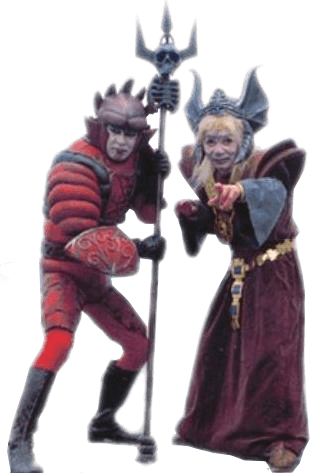
\includegraphics[width=2in]{satana11.png}
}
\end{picture}
}%
\begin{frame}
	\frametitle{Mistakes\\\begin{CJK}{UTF8}{min}間違い\end{CJK}}
	\begin{itemize}
		\item Started as a pet project
		\item Not enough strong directions
		\item Regression/Unit tests added very late
		\item Too much compromise accepted
		\item Lack of "project" communication
	\end{itemize}
\end{frame}
}

{
\usebackgroundtemplate{
\begin{picture}(0,0)
\put(200,-220){
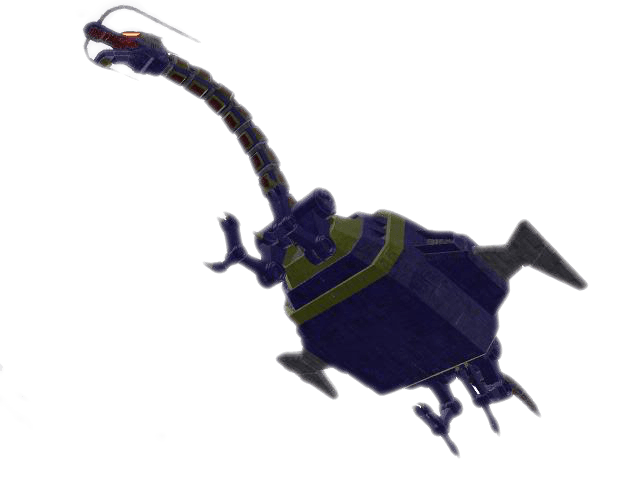
\includegraphics[width=2in]{doll1.png}
}
\end{picture}
}%
\begin{frame}
	\frametitle{Improvements\\\begin{CJK}{UTF8}{min}改善点\end{CJK}}
	\begin{itemize}
		\item Cleaning up/removing all the compatibility stuff
		\item More test driven developement
		\item Reduce the scope of what pkg(8) should do
		\item Focus on stabilising what we have
		\item Attract new developers
		\item Give more clear directions, ROADMAP
	\end{itemize}
\end{frame}
}

{
\usebackgroundtemplate{
\begin{picture}(0,0)
\put(200,-230){
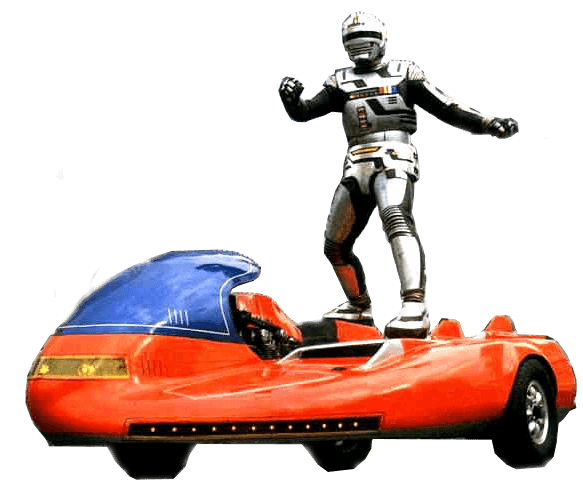
\includegraphics[width=2in]{xor-ro10.png}
}
\end{picture}
}%
\begin{frame}
	\frametitle{Roadmap\\\begin{CJK}{UTF8}{min}ロードマップ\end{CJK}}
	\begin{itemize}
		\item Provides/Requires
		\item Flexible dependencies
		\item sub packages (ports related)
		\item flavours/alternatives (ports related)
		\item List of supported ABI
		\item Maybe extensibility: plugins? lua? duktape?
		\item Transactions
		\item More regression tests
		\item 3rd party repositories:
			\begin{itemize}
				\item ports tree
				\item yum (aka linux packages)
				\item CPAN
			\end{itemize}
	\end{itemize}
\end{frame}
}

\begin{frame}
	\frametitle{New in pkg 1.5\\\begin{CJK}{UTF8}{min}pkg 1.5 変更履歴\end{CJK}}
	\begin{itemize}
		\item Improved support for NetBSD/EdgeBSD
		\item Initial support for OSX
		\item Extended credential support in plist (support for flags)
		\item 40+ new regression tests
		\item Lots of bugfixes
		\item Custom keywords can have arguments in plist
		\item Initial support for provides/requires
		\item public API now C++ friendly
	\end{itemize}
\end{frame}

\begin{frame}
	\frametitle{Packaging base\\\begin{CJK}{UTF8}{min}-> パッケージ・ベース\end{CJK}}
	\framesubtitle{Users expectations}
	\begin{itemize}
		\item Keep base as a one true entity
		\item Fine grain package to reduce security updates
		\item All options in separate packages
		\item Development tools in separate packages
		\item Ability on only install runtime things (no .a, no .h etc)
		\item Ability for developers to provide a custom repository to allow users to test their changes. Example: a new libc++
	\end{itemize}
\end{frame}

{
\usebackgroundtemplate{
\begin{picture}(0,0)
\put(200,-240){

\includegraphics[width=1.8in]{gavan_sharivan.png}
}
\end{picture}
}%
\begin{frame}
	\frametitle{Packaging base\\\begin{CJK}{UTF8}{min}パッケージ・ベース\end{CJK}}
	\begin{itemize}
		\item 4 meta packages (kernel, base, developement, debug)
		\item Fine grain small packages
		\item 3 way merge to handle /etc files
		\item Packages for RELEASES and security fixes
		\item Packages for STABLE branches
		\item Packages for HEAD
	\end{itemize}
\end{frame}
}

\begin{frame}[plain]
	\frametitle{Questions?\\\begin{CJK}{UTF8}{min}質問\end{CJK}}
	\begin{center}
		\Huge Thanks
		\\
		\Huge \begin{CJK}{UTF8}{min}ありがとう\\ございました\end{CJK}
	\end{center}
\end{frame}

\end{document}
